\documentclass[a4paper,
fontsize=11pt,
%headings=small,
oneside,
numbers=noperiodatend,
parskip=half-,
bibliography=totoc,
final
]{scrartcl}

\usepackage[babel]{csquotes}
\usepackage{synttree}
\usepackage{graphicx}
\setkeys{Gin}{width=.4\textwidth} %default pics size

\graphicspath{{./plots/}}
\usepackage[ngerman]{babel}
\usepackage[T1]{fontenc}
%\usepackage{amsmath}
\usepackage[utf8x]{inputenc}
\usepackage [hyphens]{url}
\usepackage{booktabs} 
\usepackage[left=2.4cm,right=2.4cm,top=2.3cm,bottom=2cm,includeheadfoot]{geometry}
\usepackage[labelformat=empty]{caption} % option 'labelformat=empty]' to surpress adding "Abbildung 1:" or "Figure 1" before each caption / use parameter '\captionsetup{labelformat=empty}' instead to change this for just one caption
\usepackage{eurosym}
\usepackage{multirow}
\usepackage[ngerman]{varioref}
\setcapindent{1em}
\renewcommand{\labelitemi}{--}
\usepackage{paralist}
\usepackage{pdfpages}
\usepackage{lscape}
\usepackage{float}
\usepackage{acronym}
\usepackage{eurosym}
\usepackage{longtable,lscape}
\usepackage{mathpazo}
\usepackage[normalem]{ulem} %emphasize weiterhin kursiv
\usepackage[flushmargin,ragged]{footmisc} % left align footnote
\usepackage{ccicons} 
\setcapindent{0pt} % no indentation in captions

%%%% fancy LIBREAS URL color 
\usepackage{xcolor}
\definecolor{libreas}{RGB}{112,0,0}

\usepackage{listings}

\urlstyle{same}  % don't use monospace font for urls

\usepackage[fleqn]{amsmath}

%adjust fontsize for part

\usepackage{sectsty}
\partfont{\large}

%Das BibTeX-Zeichen mit \BibTeX setzen:
\def\symbol#1{\char #1\relax}
\def\bsl{{\tt\symbol{'134}}}
\def\BibTeX{{\rm B\kern-.05em{\sc i\kern-.025em b}\kern-.08em
    T\kern-.1667em\lower.7ex\hbox{E}\kern-.125emX}}

\usepackage{fancyhdr}
\fancyhf{}
\pagestyle{fancyplain}
\fancyhead[R]{\thepage}

% make sure bookmarks are created eventough sections are not numbered!
% uncommend if sections are numbered (bookmarks created by default)
\makeatletter
\renewcommand\@seccntformat[1]{}
\makeatother

% typo setup
\clubpenalty = 10000
\widowpenalty = 10000
\displaywidowpenalty = 10000

\usepackage{hyperxmp}
\usepackage[colorlinks, linkcolor=black,citecolor=black, urlcolor=libreas,
breaklinks= true,bookmarks=true,bookmarksopen=true]{hyperref}
\usepackage{breakurl}

%meta
%meta

\fancyhead[L]{Kaden, B.\\ %author
LIBREAS. Library Ideas, 42 (2022). % journal, issue, volume.
\href{https://doi.org/10.18452/25695}{\color{black}https://doi.org/10.18452/25695}
{}} % doi 
\fancyhead[R]{\thepage} %page number
\fancyfoot[L] {\ccLogo \ccAttribution\ \href{https://creativecommons.org/licenses/by/4.0/}{\color{black}Creative Commons BY 4.0}}  %licence
\fancyfoot[R] {ISSN: 1860-7950}

\title{\LARGE{Kolumne Bibliotheksphilokartie \#2: Ein Blick nach Jüterbog}}% title
\author{Ben Kaden} % author

\setcounter{page}{1}

\hypersetup{%
      pdftitle={Kolumne Bibliotheksphilokartie \#2: Ein Blick nach Jüterbog},
      pdfauthor={Ben Kaden},
      pdfsubject={LIBREAS. Library Ideas, 42 (2022).},
      pdfkeywords={Bibliotheksbau, Postkarte, Philokartie, Öffentliche Bibliotheken,  Jüterbog},
      pdflicenseurl={https://creativecommons.org/licenses/by/4.0/},
      pdfcopyright={CC BY 4.0 International},
      pdfcontacturl={http://libreas.eu},
      pdfurl={https://doi.org/10.18452/25695},
      pdfdoi={10.18452/25695},
      pdflang={de},
      pdfmetalang={de}
     }



\date{}
\begin{document}

\maketitle
\thispagestyle{fancyplain} 

%abstracts

%body
Nach einem Ansichtskartenausflug ins kanadische Oshawa
(\url{https://doi.org/10.18452/23478}) bleiben wir diesmal
bibliophilokartistisch im Nahbereich, nämlich in Jüterbog im Fläming.
Das vorliegende Exemplar schickte mir mein Redaktionskollege Karsten
Schuldt im Juli, leider nicht aus Jüterbog selbst, sondern aus
Berlin-Neukölln. Meine Freude ist dadurch jedoch in keiner Weise
getrübt. Vielmehr freue ich mich, dass die Passion Ansichtskarte auch
innerhalb der Redaktion ein Echo findet und hoffe insgeheim auf rege
Nachahmung.

\begin{figure}
\centering
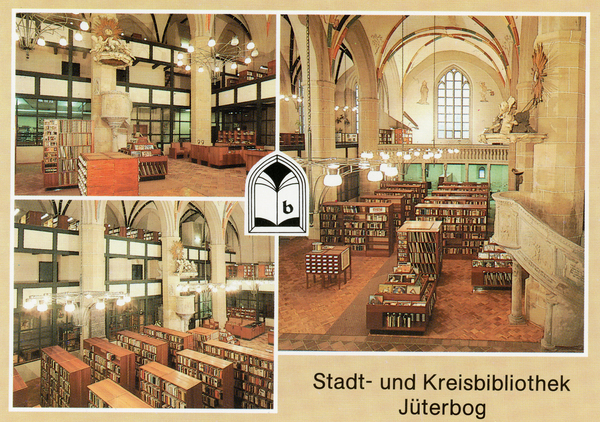
\includegraphics[width=.7\textwidth]{img/Abb1.jpg}
\caption{Abbildung 1: Ansichtskarte Stadt- und Kreisbibliothek Jüterbog.
Reichenbach (Vogtland): BILD UND HEIMAT REICHENBACH (VOGTL). Farbfotos:
Bild und Heimat (Darr), 1989. (A1/III/26/13 01 04 0844/05 K 300920/89)}
\end{figure}

Es ist ja auch ein schönes Medium, wenngleich das gezeigte Exemplar die
Designpurist*innen der Philokartie möglicherweise nicht in absolute
Verzückung versetzen wird. Die Mehrbildkarte aus dem Jahr 1989 ist
zugegeben auch weit entfernt von der kontraststarken Leistungsschau der
ostmodernen Architekturfotografie der 1960er Jahre. Sie steht für einen
Produktionstrend, der kennzeichnend für die Ansichtskartenherstellung
der DDR in den 1980er ist und einst in gewisser Weise als Schritt nach
vorn empfunden wurde. Denn lange waren Echt-Foto-Karten das Maß der
Dinge und zwar vor allem deshalb, weil sie günstiger und ohne den
Aufwand großer Druckmaschinerie hergestellt werden konnten. Ein
schlichtes Fotolabor war ausreichend. Später in der DDR kehrte sich das
mit den Fortschritten der Drucktechnologie und der Industrialisierung
der Bildproduktion um. Gerade für gewünschte größere Auflagen erwies
sich das Echt-Foto-Verfahren als unterlegen.

Der Fotograf Erasmus Schröter, in gewisser Weise der Begründer einer
spezifischen DDR-Philo\-kartie, die er freilich nie so nannte, sammelte
und verarbeitete ausschließlich Echt-Fotos und zeigt dezidiert kein
Interesse an Farb- und Mehrbildkarten.\footnote{Vergleiche Schröter,
  Erasmus: Achtzig Prozent Sonne -- Regen nie! In: Erasmus Schröter:
  Bild der Heimat. Die Echt-Foto-Postkarten aus der DDR. Berlin:
  Schwarzkopf \& Schwarzkopf, 2002.} Das ist auf den ersten, zweiten und
dritten Blick sehr nachvollziehbar, denn die zahllosen Details, die eine
raumerschließende Ansichtsfotografie so einsammelt -- ein Kind im
Sprung, ein Hund im Springbrunnen, ein Mann am Fenster --, zeigen sich
auch besser auf echten Fotografien. Bei guten Abzügen kann man die
Details bis auf Hosenträgernähe heranzoomen und sich daran die schönsten
Geschichten über das Alltagsleben der DDR oder eines der anderen Länder,
die bis in die 1980er Jahre an der Echt-Foto-Ansichtskartenkultur
festhielten, ausdenken. Gerade die für die Ansichtkartenfotografie der
DDR typische Kombination aus Inszenierungswillen und Prosaischem
bereitet den aufmerksamen Betrachter*innen den Boden, um womöglich doch
über das erstaunlichste Detail zu stolpern.

Bei den Farbdrucken bringt der Griff zur Lupe in der Regel nur eine
Annäherung an die Drucktechnik selbst. Irgendwann schaut man nur noch
ins Buntraster. Das ist bei der Postkarte hier ein wenig schade, denn
gern würde man nachvollziehen, welche Bücher und Schallplatten in die
Aufstellung in der einstigen Mönchenkirche zu Jüterbog gelangt waren.
Wobei Menschen mit einer besonderen Spezialisierung in der
DDR-Schallplattengeschichte möglicherweise auch mit dem geringem
Informationsgehalt, den die Karte bietet, anhand der Cover die
eindeutigen AMIGA-Ausgaben identifizieren können. Die viel nachgefragten
Glanzstücke des Jahres 1989 (Die Ärzte, Kylie Minogue oder gar die EPs
der Electric Beat Crew und Die Skeptiker) sind es jedenfalls nicht. Das
Jahr 1989 wäre aber auch das falsche Bezugsjahr. Denn eine
Ansichtskarte, die im Druckhaus des Hauptverlags für Ansichtskarten in
der DDR, BILD UND HEIMAT im vogtländischen Reichenbach,1989 vom Band
läuft, basiert in der Regel auf Fotografien, die etwas früher entstanden
sind. Wann allerdings Heribert Darr, Großmeister der
DDR-Ansichtskartenfotografie, hier jedoch nicht unbedingt mit seiner
beeindruckendsten Arbeit, die Stadt- und Kreisbibliothek Jüterbog
ablichtete, ist erwartungsgemäß nicht genau datierbar.

Exakt überliefert ist dagegen die Eröffnung dieses eher späten
Bibliotheksbaus der DDR.\footnote{Stadt- und Kreisbibliothek Jüterbog
  (Hrsg.), Günter Köpping: Rekonstruktion und neue Nutzung der
  ehemaligen Mönchenkirche in Jüterbog. Jüterbog, 1985} Die einst
Kirchen- und nun Bibliothekspforte öffnete sich am 5. Oktober 1985, zwei
Tage vor dem Tag der Republik, vermutlich da sich ein Sonnabend immer
besser zum feierlichen Eröffnen anbietet als ein Montag. Beeindruckend
war auf jeden Fall bereits die Tatsache der Einrichtung einer neuen
Bibliothek im Baubestand und hier sogar in einer sehr schönen
Klosterkirche aus dem frühen 16. Jahrhundert.

Einmal mehr bewies sich Jüterbog als Ort der Bibliotheksinnovation. Denn
die erste öffentliche Bibliothek des Städtchens gab es ab 1876, was in
der Region Brandenburg ein erstaunlich frühes Datum darstellt.
Schallplatten, als neues Bibliotheksmedium, konnte man seit 1971
ausleihen. Das Problem war allerdings der Platz und je größer Bestand,
Nutzung und Nutzungsvielfalt wurde, desto enger wurde es auch. Vor dem
Umzug in die Franziskanerkirche stellte man die Bestände im Rathaus der
Stadt auf knapp 200 Quadratmetern der durchaus regen Nachfrage bereit,
was bei weitem nicht den Anforderungen entsprach.

Die Möglichkeit der Nutzung der Kirche war daher für die Bibliothek eine
glückliche Fügung. Und ebenso für das Gebäude, denn die funktionale
Neuausrichtung erwies sich als Rettungsanker, den die Arbeitsgruppe
Denkmalpflege der lokalen Vertretung des Kulturbunds der DDR nun endlich
erfolgreich auswerfen konnte. Die Kirche selbst war nämlich in den
1980ern schon länger keine als solche genutzte mehr, sondern ein Lager.
Bereits in den 1970ern entstand die Idee, sie als Bibliothek zu nutzen
-- ein entsprechendes Gutachten der Denkmalpflege erklärte sie 1980 für
geeignet. Kurz darauf beschlossen die beiden maßgeblichen Räte (Kreis
und Stadt), sich auf das Projekt einzulassen.

Für die Denkmalpflege der DDR, die es lange Zeit nicht besonders einfach
bei der Rettung historischer Bausubstanz hatte, war es ein willkommener
Anwendungsfall. Das Berliner Institut für Denkmalpflege und der
entsprechende sensibilisierte und engagierte Architekt Günter Köpping,
der sich bereits ab 1961 intensiv um das Kloster Zinna bemüht hatte,
entwickelten die Pläne für den Umbau, der von einer PGH (=
Produktionsgenossenschaft des Handwerks) \enquote{V. Parteitag}
koordiniert wurde. Diese entwickelten nicht nur ein Raumkonzept für eine
Bibliothek im Baubestand, sondern konnte so auch eine Reihe von
kulturhistorisch wichtigen Details wie Epitaphen oder Deckengemälden
restaurieren.

\begin{figure}
\centering
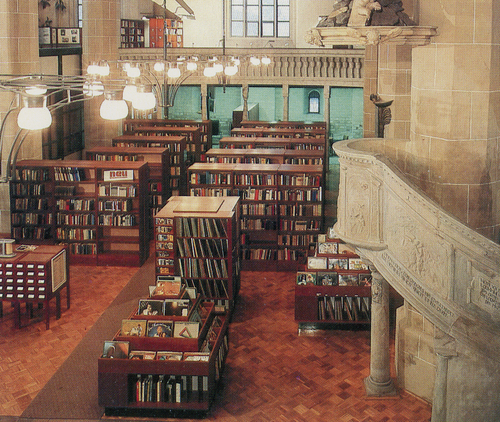
\includegraphics[width=.7\textwidth]{img/Abb2.jpg}
\caption{Abbildung 2: Ansichtskarte {[}Detail{]} Jüterbog Stadt und
Kreisbibliothek. Reichenbach (Vogtland): BILD UND HEIMAT REICHENBACH
(VOGTL). Farbfoto: Bild und Heimat (Darr), 1989. (A1/III/26/13 01 04
0844/05 K 300920/89)}
\end{figure}

Mit der auf der Karte gezeigten Phonothek wurden Ausleihe, Artothek und
Freihandbereich für die \enquote{Schöne Literatur} zentral in den
Mittelraum des Kirchengebäudes gesetzt.

Die Ansichtskartenperspektive auf die Schallplatten war aus Sicht derer,
die das Motiv in Auftrag gaben, anscheinend sogar würdig genug, um sie
parallel, also ebenfalls 1989, als Einzelbildkarte drucken zu lassen.
Beide Ausgaben erschienen unter derselben Motivdruckgenehmigungsnummer
(300920/89), was für diejenigen unter den Philokartist*innen, die ihre
Sammlung über diese vermeintlich eindeutigen Identifikatoren
erschließen, eine kleine Herausforderung darstellt. Persönlich habe ich
diese dadurch gelöst, dass ich beide Exemplare in der selben
Klarsichthülle verwahre. Für diese Kolumne bedeutet der gesonderte
größere Abzug, dass ich noch etwas tiefer in die Auflösung hinein
mikroskopieren kann.

Zurück zur Bibliothek: Unter einer Galerie integrierte man die
Kinderbibliothek, auf der Galerie die Fachliteratur sowie in einem
zweiten Galeriegeschoss ein Magazin. Auf der Ansichtskarte wirkt es fast
so, als gäbe es auch einen schönen Lesebereich an der Balustrade. Für
einige Begeisterung sorgte die Tatsache, dass im Chor der Kirche ein
\enquote{Theater der Werktätigen} untergebracht werden konnte, das uns
die Ansichtskarte leider vorenthält. Dies und auch die Tatsache, dass
mit dem Jüterboger Backsteingewölbe meines Wissens erst- und einmalig in
der DDR eine Kirche zur öffentlichen Bibliothek wurde, macht das Haus zu
einem bis heute bibliotheksarchitekturgeschichtlichen einzigartigem
Objekt.

\begin{figure}
\centering
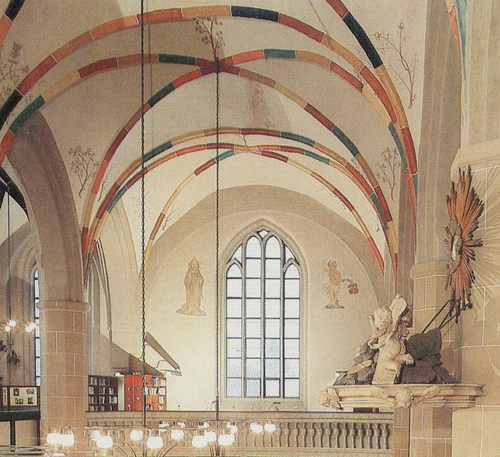
\includegraphics[width=.7\textwidth]{img/Abb3.jpg}
\caption{Abbildung 3: Ansichtskarte {[}Detail{]} Jüterbog Stadt und
Kreisbibliothek. Reichenbach (Vogtland): BILD UND HEIMAT REICHENBACH
(VOGTL). Farbfoto: Bild und Heimat (Darr), 1989. (A1/III/26/13 01 04
0844/05 K 300920/89).}
\end{figure}

Nicht ganz einzigartig, aber durchaus besonders, ist die Ansichtskarte
auch in ihrer Motivwahl. Die Ansichtskartengeschichte der DDR markiert
in der Motivgeschichte der Philokartie einen Sonderweg, denn die vielen
kleinen, wenigen mittleren und der eine ganz große Ansichtskartenverlag
des Landes inventarisierten in gewisser Weise Dorf für Dorf und Stadt
für Stadt alles, was herzeigbar war und insbesondere dann, wenn es
repräsentierte, wie sich die sozialistische Gesellschaftsform Raum gab.
Umso mehr überrascht, wie vergleichsweise selten öffentliche
Bibliotheken eine Rolle spielten. Die Berliner Staatsbibliothek und die
Leipziger Deutsche Bücherei und ein paar historische Häuser mit
übergreifender kulturgeschichtlicher Bedeutung, zum Beispiel das
Goethe-Nationalmuseum, bereichern erwartbar den bibliophilokartistischen
Kosmos. Aber die zahllosen öffentlichen Bibliotheken brauchten
vermutlich schon eine besondere städtebauliche und künstlerische
Gestaltung, wie die Bibliothek des Erfurter Neubaugebiets an der
Vilniuser Straße, um als Motiv für Postkarten herzuhalten. Dies würde
sich mit der Einschätzung des Alltagshistorikers Alf Lüdtke decken, der
für die Fotografie der DDR, zu der auch die Ansichtskartenfotografie
gehört, unter anderem eine Motivpräferenz für \enquote{bildliche
Repräsentationen der öffentlichen Sphäre, des gebauten Raumes, von
Häusern und Städten und insbesondere symbolischen Bauten}
feststellt.\footnote{Lüdtke, Alf: Kein Entkommen. Bilder-Codes und
  eigen-sinniges Fotografien. In: Karin Hartewig, Alf Lüdtke (Hrsg.):
  Die DDR im Bild. Zum Gebrauch der Fotografie im anderen deutschen
  Staat. Göttingen: Wallstein, 2004. S. 227--236.} Die großen Häuser in
Berlin und Leipzig waren als kulturgeschichtliche, teils aufgrund der
Bestände westlicher Herkunft sogar sehnsuchtsbeladenen, Leitsterne
symbolisch aufgeladen und wurden auch beispielsweise intensiv in der
erzählenden Literatur gewürdigt. Die musealen Bibliotheken gehörten zum
normalen historisch-touristischen Bildinventar wie Schlösser, Gärten und
Burgen. In ähnlicher Weise mag die eine oder andere Lesehalle eines
Kurhauses oder die Ferienbibliothek eines FDGB-Heimes zur Ehre einer
Abbildung auf einer Ansichtskarte gelangt sein. Auch der Neubau der
Berliner Stadtbibliothek mit dem berühmten A-Portal wurde auf
Ansichtskarten gewürdigt. Aber von den zahllosen kleinen
Stadtbibliotheken findet sich nur eine geringe Menge an Abbildungen auf
Ansichtskarten, gefühlt beziehungsweise sammlungsempirisch geringer noch
als dies bei Kaufhallen, Freibädern oder Polytechnischen Oberschulen der
Fall ist.

Denkbar wäre noch, dass die Überlieferung und damit heutige
Verfügbarkeit für die Motivgruppe \enquote{Öffentliche Bibliotheken} der
DDR lückenhafter ist, weil die Auflagen klein und die Identifikation,
die einem bewussten Bewahren vorausgeht, mit der eigenen Schule
möglicher größer war, als die mit der eigenen Wohngebietsbibliothek.
Dies könnte auch erklären, weshalb aus den späten 1980er Jahren und bis
1990 verstärkt BILD UND HEIMAT-Ausgaben zu öffentlichen Bibliotheken zu
finden sind. Das neue alte Haus in Jüterbog passt aber so oder so ins
Schema. Es ist repräsentativ und spielt zugleich im erwachten Zeitgeist
einer neuen Wertschätzung auch alter Bausubstanz in der DDR.

%autor

\begin{center}\rule{0.5\linewidth}{0.5pt}\end{center}

\textbf{Ben Kaden} ist Mitherausgeber von LIBREAS und beschäftigt sich
abseits seiner bibliothekswissenschaftlichen Aktivitäten zunehmend mit
dem Themenfeld der \enquote{Philokartie}. Zuletzt erschien von ihm zum Thema
die Publikation \enquote{Karten zur Ostmoderne} (Leipzig: sphere, 2020). Eine
fortlaufende Sammlungsdokumentation gibt es unter
\url{https://benkaden.tumblr.com/}.


\end{document}